\documentclass{article} % say
\usepackage{tikz}

\usetikzlibrary{arrows,decorations.pathmorphing,backgrounds,positioning,fit,calc,matrix}

\begin{document}
We are working on

\vspace{1cm}

\begin{tikzpicture}
  \draw (-1.5,0) -- (1.5,0);
  \draw (0,-1.5) -- (0,1.5);
\end{tikzpicture}.

\vspace{1cm}


% Nodes are required from below

\begin{tikzpicture}
  \draw (-1.5,0) -- (1.5,0);
  \draw (0,-1.5) -- (0,1.5);
  \draw (-1,0) .. controls (-1,0.555) and (-0.555,1) .. (0,1)
               .. controls (0.555,1) and (1,0.555) .. (1,0);
\end{tikzpicture}

\vspace{1cm}

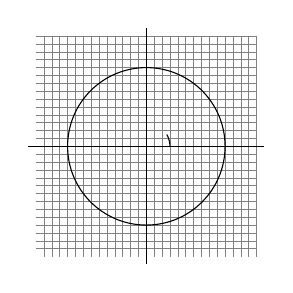
\begin{tikzpicture}
  \draw[step=.1cm,gray,very thin] (-1.4,-1.4) grid (1.4,1.4);
  \draw (-1.5,0) -- (1.5,0);
  \draw (0,-1.5) -- (0,1.5);
  \draw (0,0) circle (1cm);
  \draw (3mm,0mm) arc (0:30:3mm);
\end{tikzpicture}

\vspace{1cm}

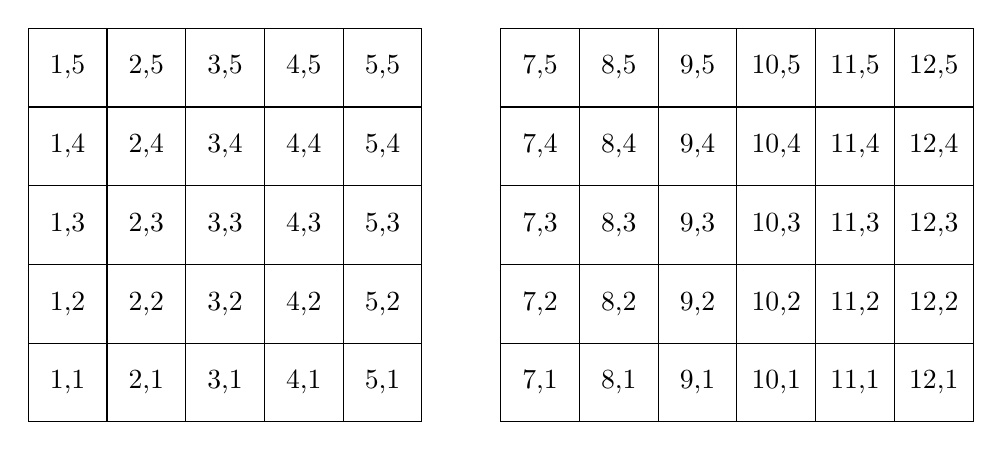
\begin{tikzpicture}
  \foreach \x in {1,2,...,5,7,8,...,12}
    \foreach \y in {1,...,5}
    {
      \draw (\x,\y) +(-.5,-.5) rectangle ++(.5,.5);
      \draw (\x,\y) node{\x,\y};
    }
\end{tikzpicture}

\vspace{1cm}


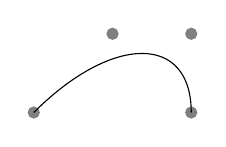
\begin{tikzpicture}
  \filldraw [gray] (0,0) circle (2pt)
                    (1,1) circle (2pt)
                    (2,1) circle (2pt)
                    (2,0) circle (2pt);
  \draw (0,0) .. controls (1,1) and (2,1) .. (2,0);
\end{tikzpicture}

\vspace{1cm}
\begin{tikzpicture}
	[kashyap/.style={help lines,color=blue!50}]
	\draw[kashyap,dashed, rotate=30] (0,0) ellipse (30mm and 15mm);
	\draw[kashyap] (3,3) ellipse (30mm and 15mm);
\end{tikzpicture}


\vspace{1cm}
\begin{tikzpicture}[scale=3]
\draw[step=0.5cm,gray,very thin] (-1.4,-1.4) grid (1.4,1.4);
\draw (-1.5,0) -- (1.5,0);
\draw (0,-1.5) -- (0,1.5);
\draw (0,0) circle (1cm);
\filldraw[fill=green!20!white, draw=green!50!black] (0,0) -- (3mm,0mm) arc (0:30:3mm) -- cycle;
\end{tikzpicture}

\vspace{1cm}
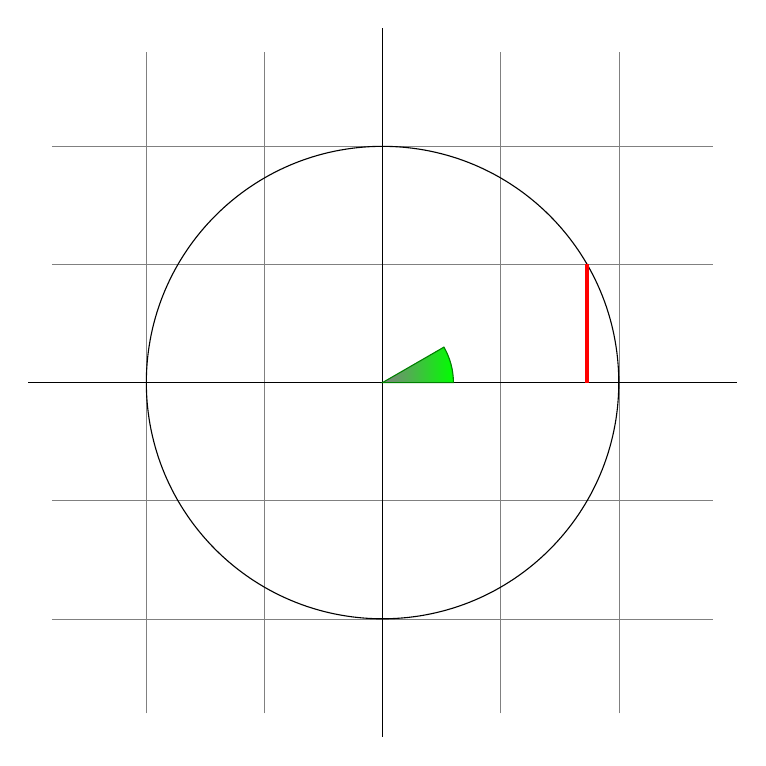
\begin{tikzpicture}[scale=3]
\draw[step=0.5cm,gray,very thin] (-1.4,-1.4) grid (1.4,1.4);
\draw (-1.5,0) -- (1.5,0);
\draw (0,-1.5) -- (0,1.5);
\draw (0,0) circle (1cm);
\shadedraw[left color=gray,right color=green, draw=green!50!black] (0,0) -- (3mm,0mm) arc (0:30:3mm) -- cycle;
\draw[red,very thick] (30:1cm) -- +(0,-0.5);
\end{tikzpicture}

\vspace{10cm}

\begin{tikzpicture}[scale=3]
  \clip (-2,-0.5) rectangle (2,1); 1 −2
  \draw[step=.5cm,gray,very thin] (-1.4,-1.4) grid (1.4,1.4);
  \filldraw[fill=green!20,draw=green!50!black] (0,0) -- (3mm,0mm) arc
  (0:30:3mm) -- cycle;
  \draw[->] (-1.5,0) -- (1.5,0) coordinate (x axis);
                                    −1
  \draw[->] (0,-1.5) -- (0,1.5) coordinate (y axis);
  \draw (0,0) circle (1cm);
  \draw[very thick,red]
    (30:1cm) -- node[left=1pt,fill=white] {$\sin \alpha$} (30:1cm |- x axis);
  \draw[very thick,blue]
    (30:1cm |- x axis) -- node[below=2pt,fill=white] {$\cos \alpha$} (0,0);
  \draw[very thick,orange] (1,0) -- node [right=1pt,fill=white]
    {$\displaystyle \tan \alpha \color{black}=
      \frac{{\color{red}\sin \alpha}}{\color{blue}\cos \alpha}$}
    (intersection of 0,0--30:1cm and 1,0--1,1) coordinate (t);
  \draw (0,0) -- (t);
  \foreach \x/\xtext in {-1, -0.5/-\frac{1}{2}, 1}
    \draw (\x cm,1pt) -- (\x cm,-1pt) node[anchor=north,fill=white] {$\xtext$};
  \foreach \y/\ytext in {-1, -0.5/-\frac{1}{2}, 0.5/\frac{1}{2}, 1}
    \draw (1pt,\y cm) -- (-1pt,\y cm) node[anchor=east,fill=white] {$\ytext$};
\end{tikzpicture}

\vspace{2cm}

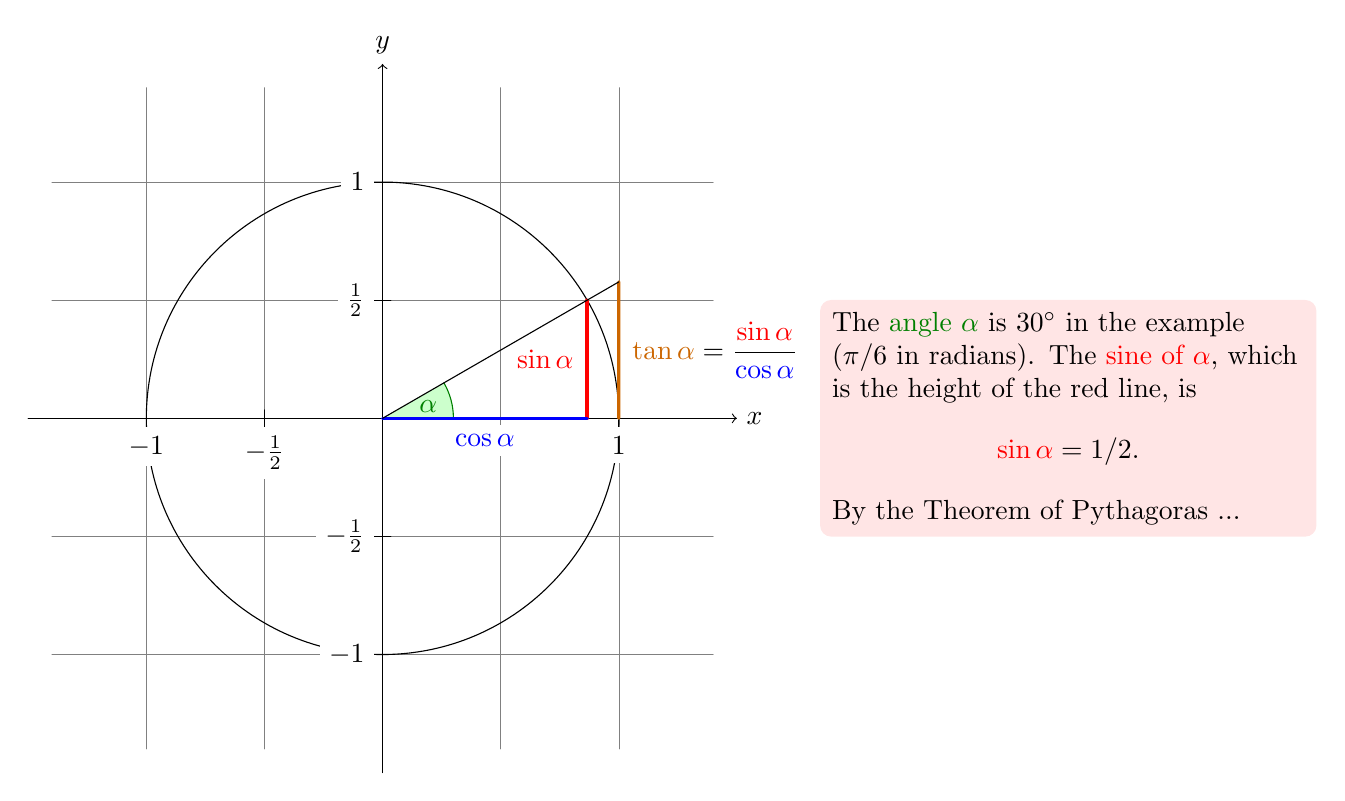
\begin{tikzpicture}
  [scale=3,line cap=round,
  % Styles
  axes/.style=,
  important line/.style={very thick},
  information text/.style={rounded corners,fill=red!10,inner sep=1ex}]
  % Local definitions
  \def\costhirty{0.8660256}
  % Colors
  \colorlet{anglecolor}{green!50!black}
  \colorlet{sincolor}{red}
  \colorlet{tancolor}{orange!80!black}
  \colorlet{coscolor}{blue}
  % The graphic
  \draw[help lines,step=0.5cm] (-1.4,-1.4) grid (1.4,1.4);
  \draw (0,0) circle (1cm);
  \begin{scope}[axes]
    \draw[->] (-1.5,0) -- (1.5,0) node[right] {$x$} coordinate(x axis);
    \draw[->] (0,-1.5) -- (0,1.5) node[above] {$y$} coordinate(y axis);
    \foreach \x/\xtext in {-1, -.5/-\frac{1}{2}, 1}
      \draw[xshift=\x cm] (0pt,1pt) -- (0pt,-1pt) node[below,fill=white] {$\xtext$};
    \foreach \y/\ytext in {-1, -.5/-\frac{1}{2}, .5/\frac{1}{2}, 1}
      \draw[yshift=\y cm] (1pt,0pt) -- (-1pt,0pt) node[left,fill=white] {$\ytext$};
  \end{scope}
  \filldraw[fill=green!20,draw=anglecolor] (0,0) -- (3mm,0pt) arc(0:30:3mm);
  \draw (15:2mm) node[anglecolor] {$\alpha$};
  \draw[important line,sincolor]
    (30:1cm) -- node[left=1pt,fill=white] {$\sin \alpha$} (30:1cm |- x axis);
  \draw[important line,coscolor]
    (30:1cm |- x axis) -- node[below=2pt,fill=white] {$\cos \alpha$} (0,0);
  \draw[important line,tancolor] (1,0) -- node[right=1pt,fill=white] {
    $\displaystyle \tan \alpha \color{black}=
    \frac{{\color{sincolor}\sin \alpha}}{\color{coscolor}\cos \alpha}$}
    (intersection of 0,0--30:1cm and 1,0--1,1) coordinate (t);
  \draw (0,0) -- (t);
  \draw[xshift=1.85cm]
    node[right,text width=6cm,information text]
    {
      The {\color{anglecolor} angle $\alpha$} is $30^\circ$ in the
      example ($\pi/6$ in radians). The {\color{sincolor}sine of
        $\alpha$}, which is the height of the red line, is
      \[
      {\color{sincolor} \sin \alpha} = 1/2.
      \]
      By the Theorem of Pythagoras ...
    };
\end{tikzpicture}


\vspace{2cm}

\begin{tikzpicture}
  \node at ( 0,2) [circle,draw] {};
  \node at ( 0,1) [circle,draw] {};
  \node at ( 0,0) [circle,draw] {};
  \node at ( 1,1) [rectangle,draw] {};
  \node at (-1,1) [rectangle,draw] {};
\end{tikzpicture}

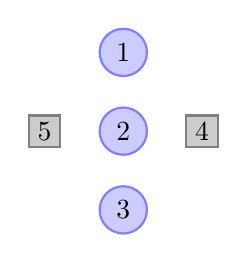
\begin{tikzpicture}
  [place/.style={circle,draw=blue!50,fill=blue!20,thick,
                  inner sep=0pt,minimum size=6mm},
   transition/.style={rectangle,draw=black!50,fill=black!20,thick,
                       inner sep=0pt,minimum size=4mm}]
  \node at ( 0,2) [place] {1};
  \node at ( 0,1) [place] {2};
  \node at ( 0,0) [place] {3};
  \node at ( 1,1) [transition] {4};
  \node at (-1,1) [transition] {5};
\end{tikzpicture}

\vspace{2cm}
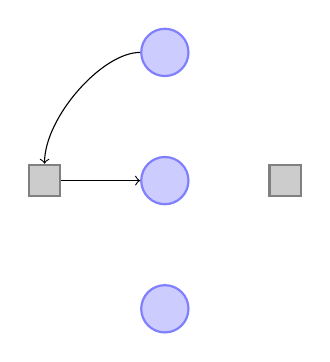
\begin{tikzpicture}
  [place/.style={circle,draw=blue!50,fill=blue!20,thick,
                  inner sep=0pt,minimum size=6mm},
   transition/.style={rectangle,draw=black!50,fill=black!20,thick,
                       inner sep=0pt,minimum size=4mm}]
  \node[place]      (waiting)                            {};
  \node[place]      (critical)       [below=of waiting] {};
  \node[place]      (semaphore)      [below=of critical] {};
  \node[transition] (leave critical) [right=of critical] {};
  \node[transition] (enter critical) [left=of critical] {};
  \draw [->] (enter critical) -- (critical);
  \draw [->] (waiting) .. controls +(left:8mm) and +(up:8mm)
                       .. (enter critical);
\end{tikzpicture}


\vspace{1cm}

                 
\begin{tikzpicture}[
nonterminal/.style={
                       rectangle,
                       minimum size=6mm,
                       very thick,
                       draw=red!50!black!50,
                       % The filling:
                       top color=white,
                       bottom color=red!50!black!20,
                       font=\itshape
                     }]
                   \node [nonterminal] {unsigned integer};
                 \end{tikzpicture}

\vspace{1cm}


          
\begin{tikzpicture}[node distance=5mm,
                     terminal/.style={
                                % The shape:
                                rectangle,minimum size=6mm,rounded corners=3mm,
                                % The rest
                                very thick,draw=black!50,
                                top color=white,bottom color=black!20,
                                font=\ttfamily}]
            \node (dot)   [terminal]                {.};
            \node (digit) [terminal,right=of dot]   {digit};
            \node (E)     [terminal,right=of digit] {E};
          \end{tikzpicture}


\vspace{1cm}


%calc is required beyond this point

          
\begin{tikzpicture}[node distance=5mm,
                     terminal/.style={
                                % The shape:
                                rectangle,minimum size=6mm,rounded corners=3mm,
                                % The rest
                                very thick,draw=black!50,
                                top color=white,bottom color=black!20,
                                font=\ttfamily}]
 \node (dot)   [terminal]                {.};
            \node (digit) [terminal,right=of dot]   {digit};
            \node (E)     [terminal,right=of digit] {E};
            \draw [help lines] let \p1 = (dot.base),
                                   \p2 = (digit.base),
                                   \p3 = (E.base)
                               in (-.5,\y1) -- (3.5,\y1)
                                  (-.5,\y2) -- (3.5,\y2)
                                  (-.5,\y3) -- (3.5,\y3);
          \end{tikzpicture}




\vspace{1cm}


\tikzset{terminal/.style={
                                % The shape:
                                rectangle,minimum size=6mm,rounded corners=3mm,
                                % The rest
                                very thick,draw=black!50,
                                top color=white,bottom color=black!20,
                                font=\ttfamily},
nonterminal/.style={
                       rectangle,
                       minimum size=6mm,
                       very thick,
                       draw=red!50!black!50,
                       % The filling:
                       top color=white,
                       bottom color=red!50!black!20,
                       font=\itshape
                     }}

\begin{tikzpicture}[node distance=5mm and 5mm]
  \node (ui1)   [nonterminal] {unsigned integer};
  \node (dot)   [terminal,right=of ui1] {.};
  \node (digit) [terminal,right=of dot] {digit};
  \node (E)     [terminal,right=of digit] {E};
  \node (plus) [terminal,above right=of E] {+};
  \node (minus) [terminal,below right=of E] {-};
  \node (ui2)   [nonterminal,below right=of plus] {unsigned integer};
\end{tikzpicture}



\vspace{1cm}
Below is done using matrix
\vspace{1cm}
%matrix library required
\begin{tikzpicture}
Below is done using matrix
  \matrix[row sep=1mm,column sep=5mm] {
    % First row:
      & & & & \node [terminal] {+}; & \\
    % Second row:
    \node [nonterminal] {unsigned integer}; &
    \node [terminal]    {.};                &
    \node [terminal]    {digit};            &
    \node [terminal]    {E};                &
                                            &
    \node [nonterminal] {hello}; \\
    % Third row:
      & & & & \node [terminal] {-}; & \\
  };
\end{tikzpicture}


\end{document}

